% !TEX program = xelatex
\documentclass[10pt,letterpaper,twocolumn]{article}

\usepackage[top=0.75in, bottom=0.75in, left=0.75in, right=0.75in]{geometry}
\usepackage{fontspec}
\usepackage{unicode-math}
\setmainfont{Latin Modern Roman}[
  Extension=.otf,
  UprightFont=lmroman10-regular,
  BoldFont=lmroman10-bold,
  ItalicFont=lmroman10-italic,
  BoldItalicFont=lmroman10-bolditalic,
]
\setsansfont{Latin Modern Sans}[
  Extension=.otf,
  UprightFont=lmsans10-regular,
  BoldFont=lmsans10-bold,
  ItalicFont=lmsans10-oblique,
  BoldItalicFont=lmsans10-boldoblique,
]
\newfontfamily\acbold{ywft-processing-bold}[Path=../../system/public/type/webfonts/,Extension=.ttf]
\setmonofont{Latin Modern Mono}[
  Extension=.otf,
  UprightFont=lmmono10-regular,
  ItalicFont=lmmono10-italic,
  Scale=0.85,
]

\usepackage{xcolor}
\usepackage{titlesec}
\usepackage{enumitem}
\usepackage{booktabs}
\usepackage{tabularx}
\usepackage{fancyhdr}
\usepackage{hyperref}
\usepackage{xurl}
\usepackage{graphicx}
\graphicspath{{figures/}{../arxiv-ac/figures/}{../arxiv-whistlegraph/figures/}{../arxiv-whistlegraph/}}
\usepackage{ragged2e}
\usepackage{microtype}
\usepackage{natbib}
\usepackage[colorspec=0.92]{draftwatermark}

\definecolor{acpink}{RGB}{180,72,135}
\definecolor{acpurple}{RGB}{120,80,180}
\definecolor{acdark}{RGB}{64,56,74}
\definecolor{acgray}{RGB}{119,119,119}
\definecolor{draftcolor}{RGB}{180,72,135}

\DraftwatermarkOptions{text=RFC DRAFT,fontsize=3cm,color=draftcolor!18,angle=45}

\hypersetup{colorlinks=true,linkcolor=acpurple,urlcolor=acpurple,citecolor=acpurple,
  pdftitle={Whistlegraph.org Funding Codes}}

\titleformat{\section}{\normalfont\bfseries\normalsize\uppercase}{\thesection.}{0.5em}{}
\titlespacing{\section}{0pt}{1.2em}{0.3em}
\titleformat{\subsection}{\normalfont\bfseries\small}{\thesubsection}{0.5em}{}
\titlespacing{\subsection}{0pt}{0.8em}{0.2em}

\pagestyle{fancy}\fancyhf{}
\renewcommand{\headrulewidth}{0pt}
\fancyhead[C]{\footnotesize\color{acpink}\textit{RFC working draft --- comments to mail@whistlegraph.org}}
\fancyfoot[C]{\footnotesize\thepage}

\newcommand{\ac}{\textsc{Aesthetic.Computer}}
\newcommand{\wg}{\textsc{Whistlegraph}}
\newcommand{\code}[1]{\texttt{#1}}

\setlist[itemize]{nosep, leftmargin=1.2em, itemsep=0.1em}
\setlist[enumerate]{nosep, leftmargin=1.4em, itemsep=0.1em}
\setlength{\columnsep}{1.8em}
\setlength{\parindent}{1em}
\setlength{\parskip}{0.3em}

\tolerance=800
\emergencystretch=1em
\hyphenpenalty=50

\begin{document}

\twocolumn[{%
\begin{center}

\includegraphics[height=4em]{pals}\par\vspace{0.5em}
{\acbold\fontsize{21pt}{25pt}\selectfont\color{acdark} Whistlegraph{\normalfont\color{acpink}.}org Funding Codes}\par
\vspace{0.45em}
{\normalfont\itshape\fontsize{11pt}{13pt}\selectfont\color{acpink} An RFC for Code-Addressed Ownership and Derivative Value Sharing on Ethereum}\par
\vspace{0.3em}
{\normalfont\fontsize{9pt}{11pt}\selectfont\color{acgray} The graphic score becomes a funding instrument: whoever holds a whistlegraph shares in the songbook that grows from it}\par
\vspace{0.6em}
{\normalsize\href{https://prompt.ac/@jeffrey}{@jeffrey}}\par
{\small\color{acgray} Aesthetic.Computer / Whistlegraph.org --- August 26, 2026}\par
{\small\color{acgray} ORCID: \href{https://orcid.org/0009-0007-4460-4913}{0009-0007-4460-4913}}\par
\vspace{0.3em}
{\small\color{acpurple} \url{https://whistlegraph.org}}\par
\vspace{0.6em}
\rule{\textwidth}{1.5pt}
\vspace{0.5em}
\end{center}

\begin{center}
{\small\color{acpink}\textbf{[ request for comments --- not for citation ]}}
\end{center}
\vspace{0.3em}

\begin{quote}
\small\noindent\textbf{Abstract.}
A whistlegraph is a graphic score that teaches you how to play it~\citep{scudder2026whistlegraph}. This RFC proposes making each score \emph{fund} what is played from it. The design assigns every whistlegraph a short code that is simultaneously its URL (\code{whistlegraph.org/imab}), its token (one ERC-721 per code), and its name (\code{imab.whistlegraph.eth}); collectors buy codes, and when Whistlegraph Dot Org releases a music track derived from a graph, the graph's current owner automatically shares in the release---a provenance citation, a first-edition claim, and a fixed split of primary mint proceeds and resale royalties. The mechanic is not speculative: an equivalent code market on Tezos produced 70 organic sales across 92 tokens in five months, with repeat collectors, but grossed roughly \$130 because the denominating asset collapsed. This proposal moves the proven mechanic to the chain with actual collector liquidity, seeds it with ten editions returning from the 2022 Feral File exhibition \emph{Ten Whistlegraphs}~\citep{feralfile2022ten}, and funds its own construction through Base's builder programs~\citep{base2026funded}. A hard boundary keeps the design out of securities territory: owners share only onchain-native value---mints, claims, royalties---never streaming revenue, and the language is patronage, never investment. Comments are invited at \href{mailto:mail@whistlegraph.org}{mail@whistlegraph.org}.
\end{quote}
\vspace{0.5em}
}]

\section{Introduction}

Between 2019 and 2023 the whistlegraph accumulated cultural value at internet scale---2.6 million TikTok followers, a New Museum commission, a Feral File exhibition, museum acquisitions---while accumulating almost no \emph{ownable} value. The form's economics ran through platforms that kept the audience and through a domain, \code{whistlegraph.com}, that lapsed and was taken by a squatter. When Feral File wrote in August 2026 to ask what should happen to the ten unsold editions it still holds,\footnote{S.~Moss-Pultz, personal communication, August 20, 2026. The message itself bounced off the lost \code{.com} domain before reaching the author---a compact demonstration of the problem this RFC addresses.} the question underneath was larger than custody: where should whistlegraphs \emph{live} so that their cultural appreciation is capturable by the people who hold them?

This RFC proposes an answer with three parts. First, an addressing scheme: every whistlegraph gets a short code that resolves identically as a web page, an ERC-721 token~\citep{eip721}, and an ENS subname~\citep{eip137}. Second, an economics: when the whistlegraph practice releases music derived from a graph---and it now releases regularly, as the artist name \emph{Whistlegraph Dot Org}---the graph's owner shares in that release through mechanisms that stay strictly onchain. Third, a funding path: the system is built on Base, whose builder programs retroactively fund exactly this category of work~\citep{base2026funded}, so construction pays for itself.

The posture throughout is \emph{request for comments}. Nothing here is deployed. The contract does not exist. The numbers that justify the design, however, are real and are reported in \S\ref{sec:evidence}.

\section{Context and Prior Work}

\subsection{The corpus}

The whistlegraph form---every drawn line is a sung line, the finished drawing is a score anyone can perform---is documented in a companion paper~\citep{scudder2026whistlegraph}. What matters for this RFC is that the corpus is large (hundreds of scores across the TikTok era), self-contained (each score is a complete work), and \emph{generative of derivatives}: scores become songs, songs become releases, releases point back at scores. A form whose works naturally spawn other works is unusually well suited to provenance-linked economics.

\begin{figure}[t]
\centering
\begin{minipage}{0.48\linewidth}
\includegraphics[width=\linewidth]{mommy-wow-score}\end{minipage}\hfill
\begin{minipage}{0.48\linewidth}
\includegraphics[width=\linewidth]{people-pleaser-score}\end{minipage}\\[2pt]
\begin{minipage}{0.48\linewidth}
\includegraphics[width=\linewidth]{puzzle-score}\end{minipage}\hfill
\begin{minipage}{0.48\linewidth}
\includegraphics[width=\linewidth]{slinky-dog-score}\end{minipage}
\caption{Four more scores from the corpus---\emph{Mommy Wow}, \emph{People Pleaser}, \emph{Puzzle}, \emph{Slinky Dog}---each a complete work, each already carrying a code on the live site (\code{w0w}, \code{ppl}, and so on), each a potential funding code.}
\label{fig:corpus}
\end{figure}

\begin{figure}[t]
\centering

\includegraphics[width=0.82\linewidth]{butterfly-cosplayer-score}
\caption{``I'm a Butterfly (Cosplayer)''---a whistlegraph graphic score. Under this proposal a score like this one carries a code that is at once its URL, its token, and its ENS name; a music release derived from it routes value to whoever holds the code.}
\label{fig:score}
\end{figure}

\subsection{Ten Whistlegraphs on Feral File}

The 2022 exhibition \emph{Ten Whistlegraphs} issued 45 sale editions across 10 works~\citep{feralfile2022ten}; its ledger records 70 edition-tokens in all. As of this draft, 45 tokens have already migrated to Ethereum---the exhibition's ERC-721 at \code{0x9294\ldots ac39}---while 25 remain on Feral File's original Bitmark-chain ledger under a single custodial address, among them the ten unsold editions now being transferred back to the practice's wallet, \code{whistlegraph.eth}, at Feral File's initiative and expense. These become the proposal's mainnet reserve tier (\S\ref{sec:system}): provenance-rich, never fire-sold, and the narrative anchor---\emph{Ten Whistlegraphs} (2022) $\rightarrow$ \emph{Funding Codes} (2026). The exhibition's collectors, meanwhile, turn out to be this proposal's most concrete asset (\S\ref{sec:network}).

\subsection{Keeps on Tezos: the mechanic, proven and punished}

From March to July 2026 the \ac{} platform ran a structurally identical market on Tezos: KidLisp pieces addressed by short \code{\$codes}, minted as FA2 tokens, sold through a purpose-built marketplace~\citep{tzkt2026keeps}. The market worked as a \emph{mechanic}---92 tokens, 70 organic sales, repeat collectors including practicing artists---and failed as a \emph{denomination}: XTZ fell to \$0.23, so five months of genuine collector demand grossed roughly \$130. Section~\ref{sec:evidence} tabulates the data. The design lesson is precise: the code-as-collectible works; put it on the chain where the collectors and the liquidity are.

\subsection{Related systems}

Code-addressed art markets are established on Ethereum: Art Blocks sells works addressed by project and mint index~\citep{artblocks2021}; fx(hash) generalized the pattern permissionlessly~\citep{fxhash2021}. Onchain royalty routing is standardized by EIP-2981~\citep{eip2981} and composable payment splitting by 0xSplits~\citep{splits2022}. The ENS specification~\citep{eip137} provides name-to-record resolution including subnames. What this proposal adds is none of those primitives but their \emph{binding}: one code addressing web, token, and name simultaneously, plus a derivative-release economics that routes new-work value to source-work owners---closer to music publishing's composition/recording split than to any existing NFT mechanic.

\section{System Design}
\label{sec:system}

\subsection{The code triple}

Each whistlegraph receives a short code---and in fact already has one: the site launched its code index in August 2026, and every score in Figure~\ref{fig:site} carries a bare bracketed code today (\code{imab} for \emph{Butterfly Cosplayer}, \code{grow} for \emph{Time To Grow}, \code{ppl} for \emph{People Pleaser}, \code{lonr} for \emph{Loner}). The code carries no sigil: the \code{\$} prefix belongs to KidLisp and its Tezos story (\S2.3), and an ENS label could not contain it anyway---a bare code keeps the triple literally identical, one string serving as path, token key, and name. The code resolves on three surfaces, and each surface verifies the others (Table~\ref{tab:triple}).

\begin{figure}[t]
\centering
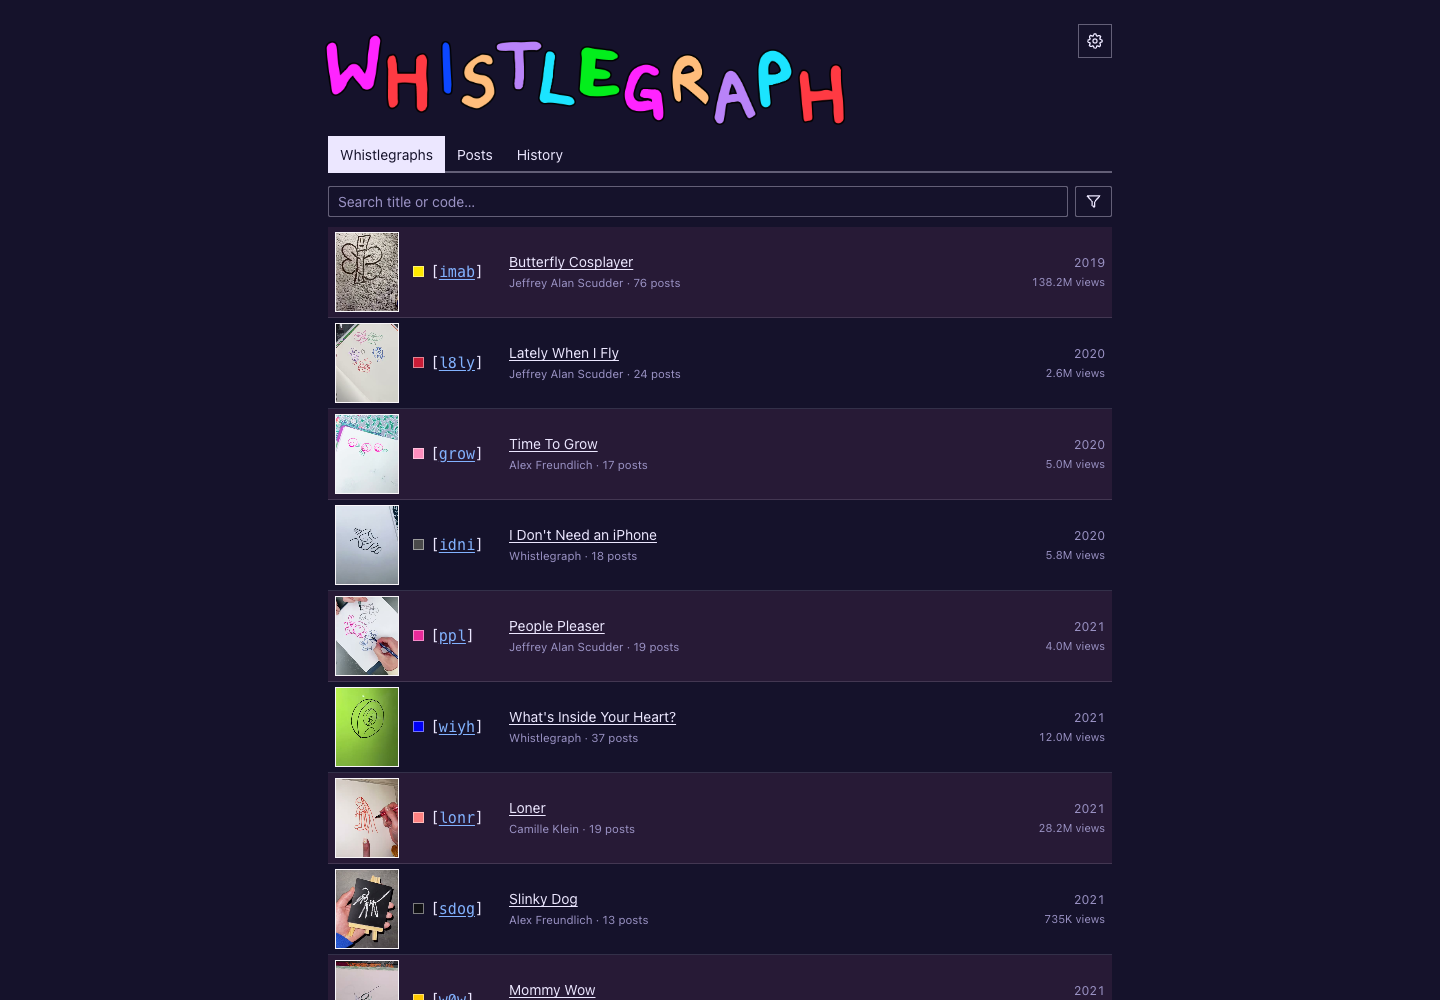
\includegraphics[width=\linewidth]{whistlegraph-org}
\caption{The live code index at \code{whistlegraph.org}, captured August 26, 2026. Every score already carries its bare code---\code{[imab]}, \code{[l8ly]}, \code{[grow]}, \code{[idni]}, \code{[ppl]}, \code{[wiyh]}, \code{[lonr]}---with per-member attribution and cumulative view counts (138.2M for \emph{Butterfly Cosplayer}). The web surface of the code triple is running; this RFC binds the token and name surfaces to it.}
\label{fig:site}
\end{figure}

\begin{table}[h]
\centering\small
\begin{tabular}{@{}lll@{}}
\toprule
\textbf{Surface} & \textbf{Resolution} & \textbf{Authority} \\
\midrule
Web & \code{whistlegraph.org/imab} & lith server \\
Token & \code{tokenId(imab)} ERC-721 & Base contract \\
Name & \code{imab.whistlegraph.eth} & ENS registry \\
\bottomrule
\end{tabular}
\caption{One code, three resolution surfaces. The site renders the score and reads ownership from the chain; the ENS parent name signs the namespace; the token's metadata URI points back at the site. Authenticity is a resolution, not a marketplace claim.}
\label{tab:triple}
\end{table}

The web surface is already live: \code{whistlegraph.org} is served by the practice's own monolith (lith) and can render scores and read chain state server-side. The name surface requires only ENS record writes---as of this draft \code{whistlegraph.eth} carries a bare address record and nothing else. The token surface is the one new artifact: a single \code{WhistlegraphCodes} ERC-721 on Base, tokenId mapped to code, mints priced in ETH from the code's own page, EIP-2981 royalties to \code{whistlegraph.eth}.

\subsection{Two tiers}

\textbf{Mainnet (reserve).} The ten returning Feral File editions land on Ethereum mainnet in \code{whistlegraph.eth}, migrating from Bitmark custody as 45 editions already have (\S2.2). They are exhibited on the site with live ownership data, relaunched deliberately during market strength, and two or three are marked permanently not-for-sale to make the remainder scarcer. They are the system's reserve asset, not its revenue.

\textbf{Base (living system).} New codes mint on Base, where transaction costs are cents, \code{ownerOf} lookups for the funding mechanics stay on one chain, and---not incidentally---a code-keyed art contract is squarely the ``novel onchain format'' that Base's retroactive Builder Grants exist to fund~\citep{base2026funded}.

\section{Funding Codes: Derivative Value Sharing}
\label{sec:funding}

The proposal's namesake mechanism. When a music release derives from graph \code{imab}, the current \code{ownerOf(imab)} receives, in escalating order of commitment (Table~\ref{tab:ladder}):

\begin{enumerate}
  \item \textbf{Provenance.} The release's metadata and page cite the source token. The graph appreciates culturally; the owner captures it on resale through standard royalties.
  \item \textbf{First edition.} The owner holds an automatic claim on edition \#1 of the release drop. A patronage perk---valuable, but promising nothing.
  \item \textbf{Mint split.} The release's primary mint proceeds and resale royalties route 80/20 between \code{whistlegraph.eth} and the graph's owner, via an 0xSplits contract resolved at drop time~\citep{splits2022}.
\end{enumerate}

\begin{table}[h]
\centering\small
\begin{tabular}{@{}llll@{}}
\toprule
\textbf{Rung} & \textbf{Owner receives} & \textbf{Rail} & \textbf{Risk} \\
\midrule
1 & provenance + resale & metadata, 2981 & none \\
2 & edition \#1 claim & claim contract & low \\
3 & 20\% of mints & 0xSplits & managed \\
\bottomrule
\end{tabular}
\caption{The value-sharing ladder. Rung 3 is the only rung that shares revenue, and it shares only onchain mint/royalty flows---never off-chain streaming income (\S\ref{sec:ethics}).}
\label{tab:ladder}
\end{table}

The closest analogy is music publishing: the graph is the \emph{composition}, the track is the \emph{recording}, and the code's owner holds something like publishing points---except the ledger is public, the split executes itself, and ``ownership'' transfers by sale of the code rather than by contract negotiation. Because the split resolves \code{ownerOf} at drop time, the value-share follows the code through secondary sales: buying a graph means buying its future first editions and splits, which is precisely why releases should make codes appreciate.

\section{Implementation Plan}

Four phases, each shippable alone.

\textbf{Phase 0 --- binding (days).} Write ENS records for \code{whistlegraph.eth} (\code{url}, avatar); publish the wallet address on the site so name and domain verify each other; register for Base Builder Rewards (prototypes qualify); receive the Feral File transfer; stand up the mainnet gallery page.

\textbf{Phase 1 --- the contract (weeks).} \code{WhistlegraphCodes} ERC-721 on Base with EIP-2981; mint page at \code{whistlegraph.org/}\textit{code}; seed the first ten codes from the TikTok-era corpus; build in public, since Base's grant scouts read the public feed.

\textbf{Phase 2 --- the first funding code.} One music release wired to one graph: first-edition claim plus the 80/20 split, released under Whistlegraph Dot Org. File the retroactive Builder Grant application on the shipped system. Pitch the whistlegraph channel to Feral File's FF1 Art Computer over the DP-1 protocol~\citep{dp1feed2025}---a paid-integration relationship that already has precedent.

\textbf{Phase 3 --- the relaunch.} The mainnet ten, told as one story: the scores come home and start funding their own songbook.

No component starts from zero: the wallet, the site, the render server, the chain-reading API keys, the FA2 contract experience, and the release pipeline all exist. The only new engineering is one Solidity contract, one claim mechanism, and ENS plumbing.

\section{Evidence}
\label{sec:evidence}

\subsection{The Tezos keeps market}

Table~\ref{tab:keeps} reports actual sales from the keeps marketplace contract, retrieved from chain indexers on August 26, 2026~\citep{tzkt2026keeps}.

\begin{table}[h]
\centering\small
\begin{tabular}{@{}llrl@{}}
\toprule
\textbf{Date} & \textbf{Code} & \textbf{Price} & \textbf{Collector} \\
\midrule
2026-07-23 & \code{\$odj} & 10.00\,\textit{tz} & edvvard.tez \\
2026-06-18 & \code{\$r94} & 14.00\,\textit{tz} & reas.tez \\
2026-06-17 & \code{\$f37} & 10.00\,\textit{tz} & nbswwit.tez \\
2026-05-31 & \code{\$wwi} & 10.00\,\textit{tz} & f3nt0n.tez \\
2026-05-23 & \code{\$pie} & 12.00\,\textit{tz} & kenconsumer.tez \\
2026-04-24 & \code{\$rip} & 8.00\,\textit{tz} & celinehen.tez \\
2026-03-30 & \code{\$noc} & 8.00\,\textit{tz} & f3nt0n.tez \\
2026-03-22 & \code{\$ex5} & 7.00\,\textit{tz} & absurdeity.tez \\
\midrule
\multicolumn{4}{@{}l@{}}{\footnotesize 70 sales all-time across 92 tokens; 5--14\,\textit{tz} range; repeat collectors.}\\
\bottomrule
\end{tabular}
\caption{Sample of organic keeps sales on Tezos (March--July 2026). The mechanic---short codes as collectible tokens---found real, repeat demand within five months of launch. At XTZ $\approx$ \$0.23, gross was only $\approx$\,\$130: proof of mechanic, indictment of denomination.}
\label{tab:keeps}
\end{table}

Two facts carry the argument. First, demand was organic and repeated---one collector bought more than a dozen codes; a well-known generative artist bought in at the top of the observed price range. Second, the dollar outcome was destroyed entirely by the denominating asset, not by the market design. A structurally identical system denominated in ETH faces collectors whose chain hosted an average \$720M of monthly NFT volume in Q1 2026~\citep{coinlaw2026nft}.

\subsection{The existing Ethereum collector network}
\label{sec:network}

The launch market is not hypothetical either---it can be enumerated. Reading the exhibition's ledger through the Feral File API and probing each holder through a chain indexer (August 26, 2026) yields the network in Figure~\ref{fig:network}: \textbf{17 Ethereum addresses hold the 45 migrated editions} of \emph{Ten Whistlegraphs} on the exhibition contract. The distribution is a classic collector pyramid---two full sets of all ten works (consistent with artist or insider sets), one eight-edition collector, and fourteen holders of one or two editions each.

More important than the holdings is the pulse: \textbf{six of the seventeen acquired an NFT within the last twelve months, three of them within the last ninety days.} These are live wallets, already provenance-linked to the whistlegraph corpus, whose addresses are known---the natural first-notification list for a funding-code drop. The Tezos keeps collectors (\S6.1) form a second seed cohort on the other chain. A launch, in other words, begins with a mapped audience rather than a cold market: the same method (ledger $\rightarrow$ owner set $\rightarrow$ activity probe) reruns in one script whenever the list needs refreshing.

\begin{figure}[t]
\centering
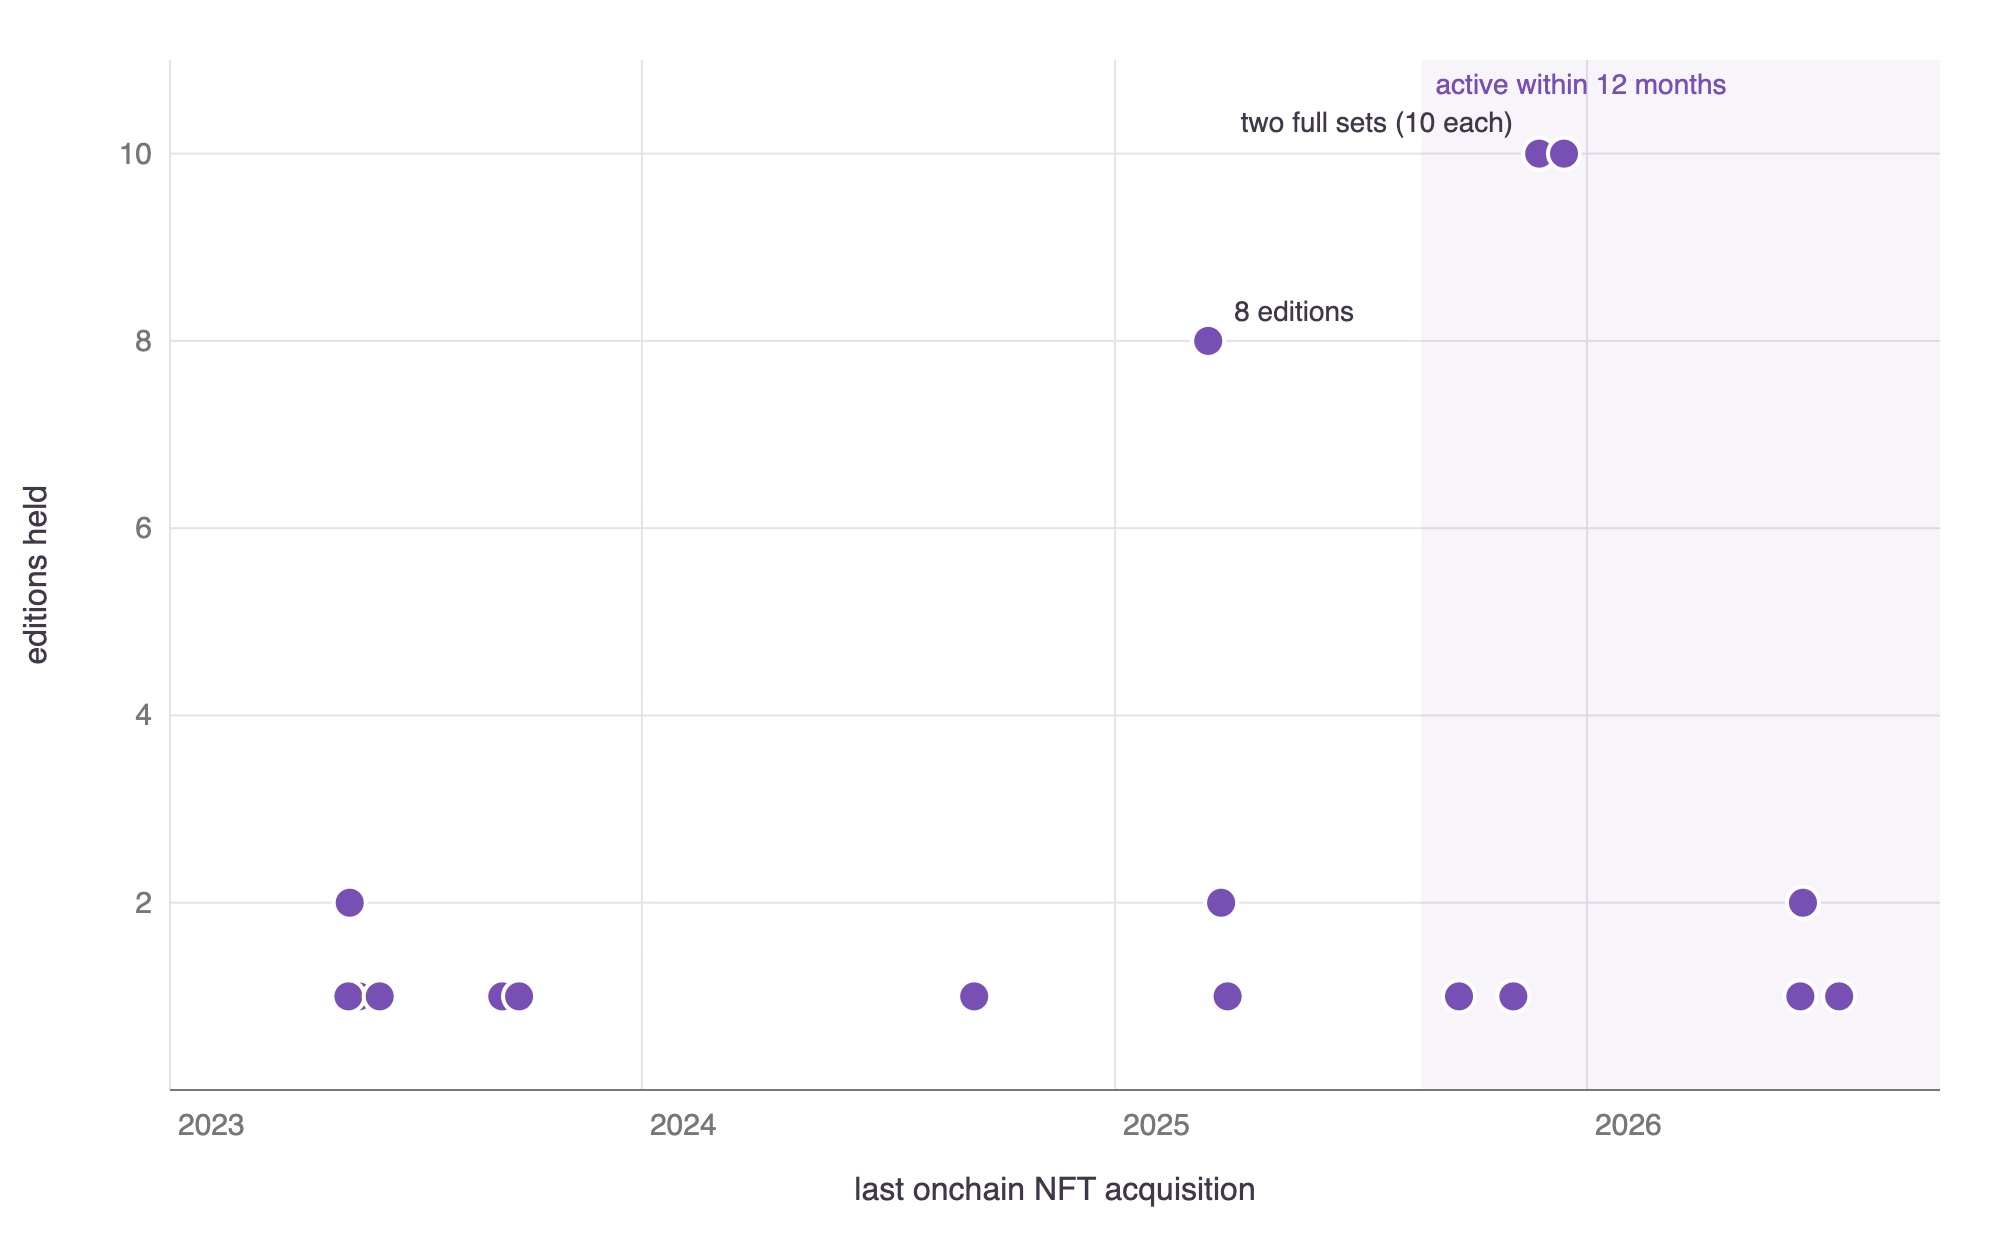
\includegraphics[width=\linewidth]{collector-map}
\caption{The existing Ethereum collector network of \emph{Ten Whistlegraphs}: one dot per holding address (n=17, jittered where coincident), positioned by its most recent onchain NFT acquisition and the number of editions held. The shaded band marks activity within the twelve months preceding this draft; six of seventeen wallets fall inside it. Data: Feral File exhibition ledger + Alchemy transfer index, 2026-08-26.}
\label{fig:network}
\end{figure}

\subsection{Market timing}

As of this draft ETH trades near \$2{,}500 after a sharp August advance driven by spot-ETF inflows, and art-market volume is rebounding from its 2024 trough~\citep{coinlaw2026nft}. Rallies are when collectors spend and when builder programs are generous; the implementation plan's Phase 0--1 window is deliberately aligned with one.

\section{Ethics, Legal, and Limitations}
\label{sec:ethics}

\textbf{The securities boundary.} A promise that buyers will profit from the efforts of others is the core of the \emph{Howey} investment-contract test~\citep{howey1946}. This design therefore shares only onchain-native value---mints, claims, resale royalties---and never tokenizes off-chain income such as streaming or distribution revenue. Public language is patronage language (``the owner receives the first edition and a royalty split''), never return language (``invest to earn''). Any copy describing rung 3 of the ladder receives legal review before shipping. If counsel finds rung 3 unsafe as designed, rungs 1--2 stand alone.

\textbf{Concentration risks.} The system is one artist's practice: key custody, release cadence, and the site are single points of failure. Mitigations are boring and listed: hardware custody for \code{whistlegraph.eth}, the domain renewal on a tracked deadline (the \code{.com} loss is the cautionary tale), and contract immutability so tokens survive the site.

\textbf{Chain dependence.} The Tezos episode shows the design's exposure to its denominating asset. ETH concentration is a judgment call, not a hedge; the split design keeps functioning at any price, but dollar outcomes will ride the chain.

\textbf{Energy.} All target chains are proof-of-stake; the footprint of minting is negligible relative to the practice's video production.

\textbf{What this is not.} Not a DAO, not a token launch, not fractionalization of the artworks themselves. Codes are whole works with whole owners.

\section{Conclusion}

The whistlegraph began as a score that teaches you how to play it. This RFC extends the same reflexivity to its economics: a score that funds what is played from it. The addressing is one code across web, token, and name; the economics is a three-rung ladder that routes derivative value to source owners without crossing the securities line; the evidence is a five-month, 70-sale field trial that proved the mechanic and burned the denomination; and the construction is designed to be paid for by the ecosystem it lands in. The ten editions returning from Feral File make the timing concrete: the scores are coming home, and this is the proposal for what they do when they arrive.

Comments---mechanism-design objections, legal caution, collector perspective, prior art---are invited at \href{mailto:mail@whistlegraph.org}{mail@whistlegraph.org}.

\vspace{0.5em}
\noindent{\small\color{acgray}\textit{Platter consulted: the Whistlegraph paper and platter, the keeps marketplace chain data, the Feral File correspondence, \code{reports/whistlegraph-org-funding-codes.md}, and the Base, ENS, and EIP specifications cited below.}}

\vspace{0.5em}
\noindent\textbf{ORCID:} \href{https://orcid.org/0009-0007-4460-4913}{0009-0007-4460-4913}

\def\bibfont{\footnotesize}
\setlength{\bibsep}{0.25em}
\bibliographystyle{plainnat}
\bibliography{references}

\end{document}
